%
%  =======================================================================
%  ····Y88b···d88P················888b·····d888·d8b·······················
%  ·····Y88b·d88P·················8888b···d8888·Y8P·······················
%  ······Y88o88P··················88888b·d88888···························
%  ·······Y888P··8888b···88888b···888Y88888P888·888·88888b·····d88b·······
%  ········888······"88b·888·"88b·888·Y888P·888·888·888·"88b·d88P"88b·····
%  ········888···d888888·888··888·888··Y8P··888·888·888··888·888··888·····
%  ········888··888··888·888··888·888···"···888·888·888··888·Y88b·888·····
%  ········888··"Y888888·888··888·888·······888·888·888··888··"Y88888·····
%  ·······························································888·····
%  ··························································Y8b·d88P·····
%  ···························································"Y88P"······
%  =======================================================================
% 
%  -----------------------------------------------------------------------
% Author       : 焱铭
% Date         : 2023-07-04 20:57:38 +0800
% LastEditTime : 2023-07-04 21:44:56 +0800
% Github       : https://github.com/YanMing-lxb/
% FilePath     : \multi-objective_optimization_microchannel_heat_sink-with_embedded_module_with_ribs_and_pin-fins\Section\Section2.tex
% Description  : 
%  -----------------------------------------------------------------------
%

\section{Mathematical modeling of the microchannel heat sink}

\cref{fig:structure} shows the schematic design of MCHS-SR and the proposed MCHS-RPFEM.


\begin{figure*}[htbp] % figure* 可进行跨栏
    \centering % 居中
    \scriptsize % 设置字体
    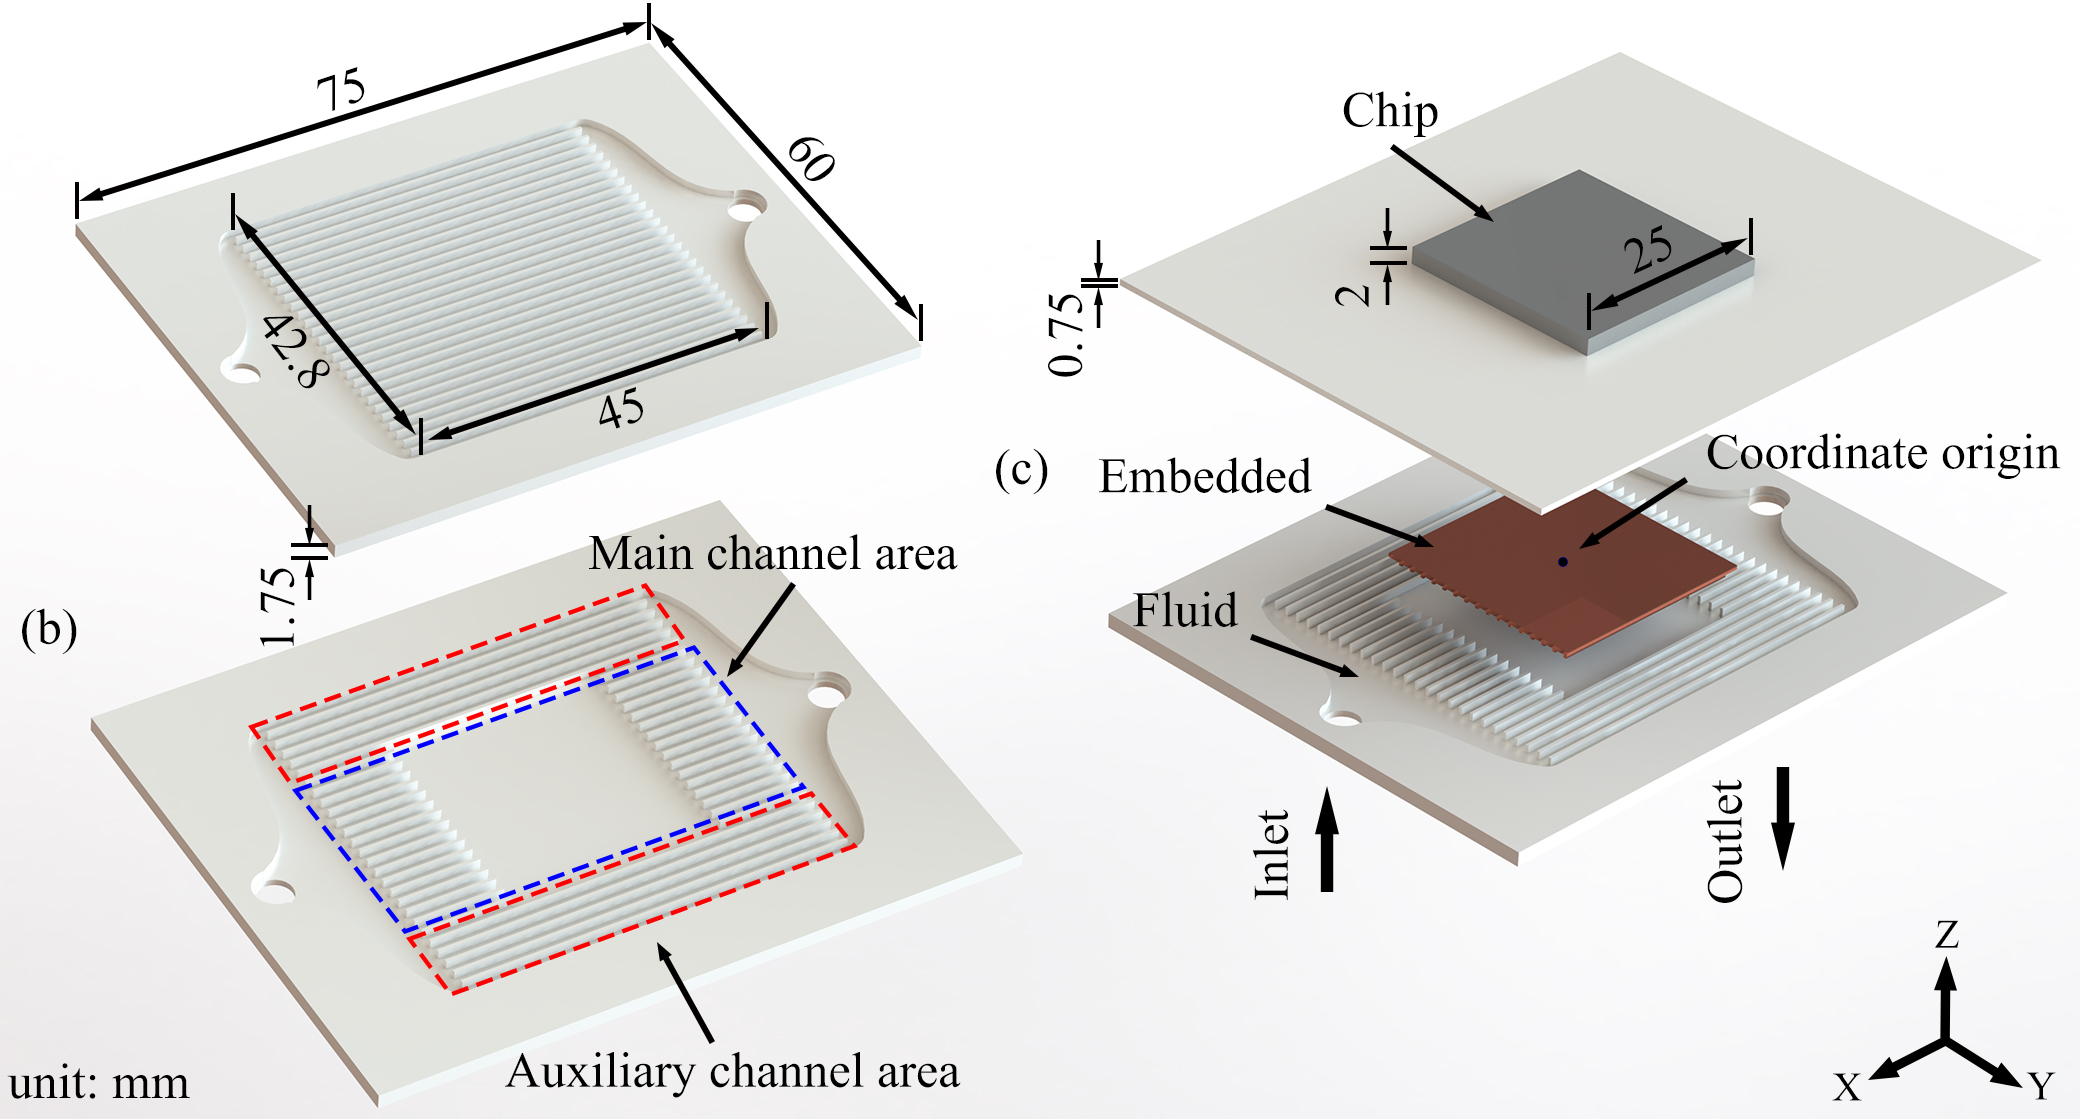
\includegraphics[width=1 \textwidth]{Schematic.jpg} % 
    \caption{
        (a) Straight rectangular microchannel (MCHS-SR),
        (b) microchannel heat sink with embedded modules with ribs and pin-fins (MCHS-RPFEM),
        (c) schematic diagram of the structure of MCHS-RPFEM.}
    \label{fig:structure}
\end{figure*}
Embedded module with ribs and pin-fins embedded in microchannel heat sink below chip.
\cref{tab:structure-parameter} shows the geometric parameters of the embedded module.
To investigate the effect of ribs and pin-fins on fluid flow and heat transfer on the embedded module in MCHS-RPFEM, three parameters were selected to be varied.
These three parameters are relative rib height ($\alpha$), relative pin-fin height ($\beta)$, and relative number of auxiliary channels ($\gamma$).

\begin{table}[htbp]
    \centering
    \scriptsize
    \caption{MCHS-RPFEM geometric parameter table}
    \begin{tabular}{lccccccc}
        \toprule
        Geometrical parameters & $W_{rib}$ & $H_{rib}$ & $d_{rib}$ & $S_{pf}$ & $H_{pf}$ & $H_{ch}$ \\
        \midrule
        Value, $\mu m$         & 400       & 1000      & 1600      & 300      & 1000     & 1000     \\
        \bottomrule
    \end{tabular}
    \label{tab:structure-parameter}
\end{table}